O sinal retangular bipolar vale $-A$ fora do pulso e $A$ durante o pulso.
Com os mesmos intervalos do sinal 7, sendo assim, esse sinal pode ser representado 
pela equação \ref{eq:retangular_bipolar_variavel}.
\begin{equation}
    \begin{aligned}
        v_8(x)&=\begin{cases}
            -A, & 0\leq x<\phi, \\
            A, & \phi\leq x<\phi+d, \\
            -A, & \phi+d\leq x<P,
        \end{cases} \\
        v_8(x+P)&=v_8(x), \qquad v_8(x)=2v_7(x)-A.
    \end{aligned}
    \label{eq:retangular_bipolar_variavel}
\end{equation}

Ao integrar os três intervalos em um período, obtém-se a média, ou seja, $a_0^{(8)}$. 
\begin{equation}
    \begin{aligned}
        a_0^{(8)}&=\frac{1}{P}\biggl[
            -A\phi+Ad-A(P-\phi-d)\biggr] \\
            &=\frac{2Ad-AP}{P}=A(2D-1).
    \end{aligned}
\end{equation}

Calculando os coeficientes de Fourier desse sinal, obtém-se:
\begin{equation}
    \begin{aligned}
        a_n^{(8)}&=\frac{2}{P}\int_0^P[2v_7(x)-A]\cos(k_nx)\,dx \\
            &=\frac{4A}{P}\int_\phi^{\phi+d}\cos(k_nx)\,dx \\
            &=\frac{4A}{Pk_n}[\sin(k_nx)]_\phi^{\phi+d} \\
            &=\frac{4A}{\pi n}\sin(\pi nD)\cos(k_nm),
    \end{aligned}
\end{equation}
\begin{equation}
    \begin{aligned}
        b_n^{(8)}&=\frac{4A}{P}\int_\phi^{\phi+d}\sin(k_nx)\,dx \\
            &=-\frac{4A}{Pk_n}[\cos(k_nx)]_\phi^{\phi+d} \\
            &=\frac{4A}{\pi n}\sin(\pi nD)\sin(k_nm).
    \end{aligned}
\end{equation}

Ao analisar os resultados obtidos, percebe-se que os coeficientes do sinal retangular bipolar são o dobro dos coeficientes do sinal retangular unipolar, ou seja, $a_n^{(8)}=2a_n^{(7)}$ e $b_n^{(8)}=2b_n^{(7)}$.
Além disso, a amplitude de cada harmônica é dada por:

\begin{equation}
    \begin{aligned}
        C_n^{(8)}&=\frac{4A}{\pi n}\lvert\sin(\pi nD)\rvert.
    \end{aligned}
\end{equation}

Para $\phi=\theta$, $m=P/2$ e os coeficientes se reduzem aos apresentados na equação \ref{eq:coefi_retangular_bipolar_variavel}.
\begin{equation}
    \begin{aligned}
        a_0^{(8)}&=A(2D-1), \\
        a_n^{(8)}&=\frac{4A}{\pi n}(-1)^n\sin(\pi nD), \\
        b_n^{(8)}&=0.
    \end{aligned}
    \label{eq:coefi_retangular_bipolar_variavel}
\end{equation}

Para $\phi\neq\theta$, utilizam-se as expressões gerais acima.
Um deslocamento do pulso com $D$ fixo modifica a fase, mas preserva $C_n$.

\subsubsection{Reconstruções dos sinais retangulares com série de Fourier até a ordem 7}

Pela identidade trigonométrica $\cos(u-v)=\cos u\cos v+\sin u\sin v$,
as duas reconstruções, para qualquer centro $m$, são:
\begin{equation}
    \begin{aligned}
        v_{7,7}(x)&=AD+\frac{2A}{\pi}\sum_{n=1}^{7}
            \frac{\sin(\pi nD)}{n} \\
            &\qquad\qquad {}\times\cos[k_n(x-m)], \\
        v_{8,7}(x)&=A(2D-1)+\frac{4A}{\pi}\sum_{n=1}^{7}
            \frac{\sin(\pi nD)}{n} \\
            &\qquad\qquad {}\times\cos[k_n(x-m)].
    \end{aligned}
    \label{eq:retangulares_7}
\end{equation}

Esses somatórios incluem explicitamente as ordens $1,2,\ldots,7$.
Para ilustrar $\phi=\theta$, pode-se adotar $d=P/3$ e $\phi=\theta=P/3$.
Então $D=1/3$, $m=P/2$. Assim, tem-se para esse exemplo os coeficientes de ordem 1 e 2:
\begin{equation}
    \begin{aligned}
        a_1^{(7)}&=\frac{2A}{\pi}(-1)\sin\frac{\pi}{3}
            =-\frac{\sqrt{3}A}{\pi}, \\
        a_2^{(7)}&=\frac{2A}{2\pi}\sin\frac{2\pi}{3}
            =\frac{\sqrt{3}A}{2\pi}.
    \end{aligned}
\end{equation}

As ordens 3 e 6 são nulas. A expansão completa desse exemplo é:
\begin{equation}
    \begin{aligned}
        v_{7,7}(x)&=\frac{A}{3}-\frac{\sqrt{3}A}{\pi}\biggl[
            \cos(k_1x)-\frac{\cos(k_2x)}{2} \\
            &\qquad {}+\frac{\cos(k_4x)}{4}
            -\frac{\cos(k_5x)}{5}+\frac{\cos(k_7x)}{7}\biggr], \\
        v_{8,7}(x)&=2v_{7,7}(x)-A.
    \end{aligned}
\end{equation}

Considerando um exemplo para $\phi\neq\theta$, mantendo $d=P/3$, mas escolhendo $\phi=P/6$ e
$\theta=P/2$. Escolhendo, também, $m=P/3$ para a componente fundamental, tem-se os coeficientes de ordem 1:

\begin{equation}
    \begin{aligned}
        a_1^{(7)}&=\frac{2A}{\pi}\sin\frac{\pi}{3}\cos\frac{2\pi}{3}
            =-\frac{\sqrt{3}A}{2\pi}, \\
        b_1^{(7)}&=\frac{2A}{\pi}\sin\frac{\pi}{3}\sin\frac{2\pi}{3}
            =\frac{3A}{2\pi}, \\
        C_1^{(7)}&=\sqrt{\frac{3A^2}{4\pi^2}+\frac{9A^2}{4\pi^2}}
            =\frac{\sqrt{3}A}{\pi}.
    \end{aligned}
\end{equation}

As Tabelas \ref{tab:ret1} e \ref{tab:ret2} apresentam todas as ordens
desses exemplos. Os coeficientes bipolares são o dobro dos unipolares;
as médias são $A/3$ e $-A/3$, respectivamente.
\begin{table}[H]
\centering\small
\setlength{\tabcolsep}{3.5pt}
\caption{Coeficientes teóricos unipolares do exemplo simétrico, divididos por $A$.}\label{tab:ret1}
\begin{tabular}{crr}\hline
$n$ & $a_n/A$ & $b_n/A$ \\ \hline
1 & $-0{,}551329$ & $0{,}000000$ \\
2 & $0{,}275664$ & $0{,}000000$ \\
3 & $0{,}000000$ & $0{,}000000$ \\
4 & $-0{,}137832$ & $0{,}000000$ \\
5 & $0{,}110266$ & $0{,}000000$ \\
6 & $0{,}000000$ & $0{,}000000$ \\
7 & $-0{,}078761$ & $0{,}000000$ \\
\hline\end{tabular}
\end{table}

\begin{table}[H]
\centering\small
\setlength{\tabcolsep}{3.5pt}
\caption{Coeficientes teóricos unipolares do exemplo assimétrico, divididos por $A$.}\label{tab:ret2}
\begin{tabular}{crr}\hline
$n$ & $a_n/A$ & $b_n/A$ \\ \hline
1 & $-0{,}275664$ & $0{,}477465$ \\
2 & $-0{,}137832$ & $-0{,}238732$ \\
3 & $0{,}000000$ & $0{,}000000$ \\
4 & $0{,}068916$ & $-0{,}119366$ \\
5 & $0{,}055133$ & $0{,}095493$ \\
6 & $0{,}000000$ & $0{,}000000$ \\
7 & $-0{,}039381$ & $0{,}068209$ \\
\hline\end{tabular}
\end{table}


\subsubsection{Dois ciclos retangulares alternados}
A partir das figuras \ref{fig:sinal_retangular_unipolar} e\ref{fig:sinal_retangular_bipolar}, adotou-se a hipótese de que esse par se repete, com as condições apresentadas abaixo:

\begin{equation}
    \begin{aligned}
        P&=\phi+d+\theta=\phi'+d'+\theta', \\
        L&=2P, \qquad k_n=\frac{n\pi}{P}, \\
        \ell_1&=\phi, \qquad r_1=\phi+d, \\
        \ell_2&=P+\phi', \qquad r_2=P+\phi'+d'.
    \end{aligned}
\end{equation}

No intervalo $0\leq x<2P$, $v_{7,2P}$ vale $A$ em
$[\ell_1,r_1)$ e $[\ell_2,r_2)$ e zero no restante; sua extensão é
periódica. O bipolar é $v_{8,2P}=2v_{7,2P}-A$. Se o par não se repetir,
esses parâmetros, isoladamente, não definem um sinal periódico.

Calculando os coeficientes de Fourier para o sinal unipolar, obtém-se:
\begin{equation}
    \begin{aligned}
        a_{0,2P}^{(7)}&=\frac{A}{2P}\sum_{j=1}^{2}\int_{\ell_j}^{r_j}\!dx
            =\frac{A(d+d')}{2P}, \\
        a_{n,2P}^{(7)}&=\frac{A}{P}\sum_{j=1}^{2}
            \int_{\ell_j}^{r_j}\cos(k_nx)\,dx \\
            &=\frac{A}{\pi n}\sum_{j=1}^{2}
                [\sin(k_nr_j)-\sin(k_n\ell_j)], \\
        b_{n,2P}^{(7)}&=\frac{A}{P}\sum_{j=1}^{2}
            \int_{\ell_j}^{r_j}\sin(k_nx)\,dx \\
            &=\frac{A}{\pi n}\sum_{j=1}^{2}
                [\cos(k_n\ell_j)-\cos(k_nr_j)].
    \end{aligned}
\end{equation}

Já para o sinal bipolar, obtém-se:
\begin{equation}
    \begin{aligned}
        a_{0,2P}^{(8)}&=A\left(\frac{d+d'}{P}-1\right), \\
        a_{n,2P}^{(8)}&=2a_{n,2P}^{(7)}, \qquad
        b_{n,2P}^{(8)}=2b_{n,2P}^{(7)}.
    \end{aligned}
\end{equation}

As reconstruções, por meio da série de Fourier,são obtidas somando $n=1,\ldots,7$ na
equação \ref{eq:convencao_fourier}, agora com $L=2P$.
Neste caso, a frequência fundamental é $f_0=\omega/(2P)$, desde que
$2P$ seja o menor período. Se os dois ciclos coincidirem, o período
mínimo volta a $P$ e as ordens ímpares da base $2P$ se anulam.

No exemplo $\phi=P/6$, $d=P/3$, $\theta=P/2$,
$\phi'=P/4$, $d'=P/2$ e $\theta'=P/4$, obtém-se
\begin{equation}
    \begin{aligned}
        a_{0,2P}^{(7)}&=\frac{5A}{12}, \qquad
        a_{0,2P}^{(8)}=-\frac{A}{6}, \\
        a_{1,2P}^{(7)}&=\frac{A}{\pi}\biggl[
            \sin\frac{\pi}{2}-\sin\frac{\pi}{6} \\
            &\qquad {}+\sin\frac{7\pi}{4}-\sin\frac{5\pi}{4}\biggr]
            =\frac{A}{2\pi}, \\
        b_{1,2P}^{(7)}&=\frac{A}{\pi}\biggl[
            \cos\frac{\pi}{6}-\cos\frac{\pi}{2} \\
            &\qquad {}+\cos\frac{5\pi}{4}-\cos\frac{7\pi}{4}\biggr] \\
            &=\frac{A}{\pi}\left(\frac{\sqrt{3}}{2}-\sqrt{2}\right).
    \end{aligned}
\end{equation}

Todas as sete ordens para reconstrução do sinal estão na Tabela \ref{tab:ret3}.
\begin{table}[H]
\centering
\small\setlength{\tabcolsep}{3.5pt}
\caption{Coeficientes teóricos unipolares do exemplo com dois ciclos alternados, divididos por $A$.}\label{tab:ret3}
\begin{tabular}{crr}\hline
$n$ & $a_n/A$ & $b_n/A$ \\ \hline
1 & $0{,}159155$ & $-0{,}174494$ \\
2 & $-0{,}456142$ & $0{,}238732$ \\
3 & $-0{,}212207$ & $0{,}150053$ \\
4 & $-0{,}068916$ & $-0{,}119366$ \\
5 & $0{,}031831$ & $0{,}034899$ \\
6 & $0{,}106103$ & $0{,}000000$ \\
7 & $-0{,}022736$ & $-0{,}103689$ \\
\hline\end{tabular}
\end{table}


\subsection{Ondas deslocadas e alteração do período}
\begin{figure}[H]
    \centering
    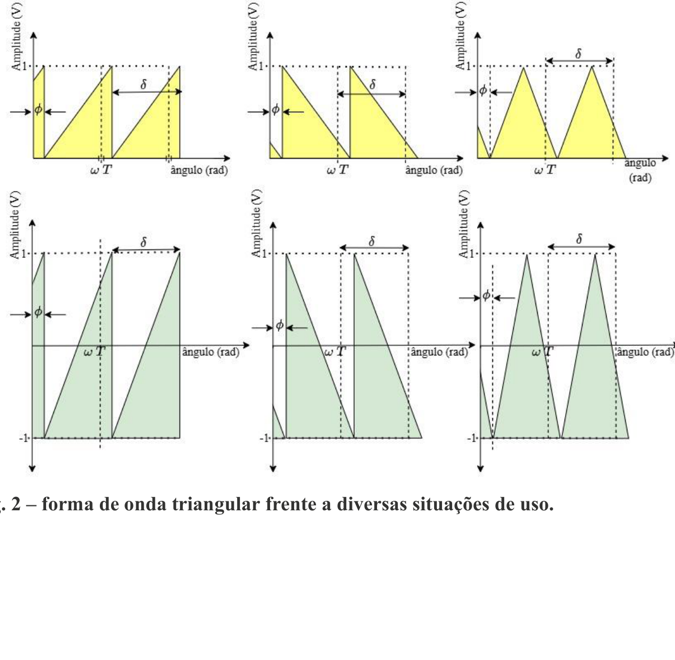
\includegraphics[width=\linewidth]{images/figura2_memorial-000.png}
\caption{Seis formas de onda da Figura 2 do enunciado.}
    \label{fig:ondas_deslocadas}
\end{figure}

Para representar as seis ondas da figura \ref{fig:ondas_deslocadas},
adota-se $\phi$ como deslocamento angular e $\delta>0$ como período
efetivo. Além disso, define-se:
\begin{equation}
    u_\delta(x)=\frac{\operatorname{mod}(x-\phi,\delta)}{\delta},
    \qquad 0\leq u_\delta<1.
\end{equation}

As equações completas dos sinais, incluindo a periodicidade, são:
\begin{equation}
    \begin{aligned}
        \widetilde v_1(x)&=Au_\delta, \\
        \widetilde v_2(x)&=A(1-u_\delta), \\
        \widetilde v_3(x)&=A\left(1-2\left|u_\delta-\frac12\right|\right), \\
        \widetilde v_4(x)&=A(2u_\delta-1), \\
        \widetilde v_5(x)&=A(1-2u_\delta), \\
        \widetilde v_6(x)&=A\left(1-4\left|u_\delta-\frac12\right|\right).
    \end{aligned}
\end{equation}

\subsubsection{Derivação dos coeficientes deslocados}
Sejam $a_{n,0}$ e $b_{n,0}$ os coeficientes sem deslocamento, já
recalculados na base de período $\delta$. Escrevendo
$q_n=2\pi n/\delta$ e $\psi=2\pi\phi/\delta$,

\begin{equation}
    \begin{aligned}
        \cos[q_n(x-\phi)]&=\cos(q_nx)\cos(n\psi) \\
            &\quad {}+\sin(q_nx)\sin(n\psi), \\
        \sin[q_n(x-\phi)]&=\sin(q_nx)\cos(n\psi) \\
            &\quad {}-\cos(q_nx)\sin(n\psi).
    \end{aligned}
\end{equation}

Multiplicando pelos coeficientes e agrupando seno e cosseno,
\begin{equation}
    \begin{aligned}
        \widetilde a_n&=a_{n,0}\cos(n\psi)-b_{n,0}\sin(n\psi), \\
        \widetilde b_n&=a_{n,0}\sin(n\psi)+b_{n,0}\cos(n\psi).
    \end{aligned}
    \label{eq:rotacao_coeficientes}
\end{equation}

A média não muda. Elevando ao quadrado e somando, os termos cruzados
se cancelam:
\begin{equation}
    \begin{aligned}
        \widetilde a_n^2+\widetilde b_n^2
            &=(a_{n,0}^2+b_{n,0}^2) \\
            &\quad {}\times[\cos^2(n\psi)+\sin^2(n\psi)] \\
            &=a_{n,0}^2+b_{n,0}^2.
    \end{aligned}
\end{equation}

Portanto, deslocar a onda preserva cada amplitude e energia harmônica.
Definindo $r_n=A/(\pi n)$ e $h_n=2A[(-1)^n-1]/(\pi^2n^2)$,
as seis substituições estão na Tabela \ref{tab:deslocamentos}.
\begin{table}[H]
    \centering\small
    \caption{Coeficientes das seis ondas deslocadas, $n=1,\ldots,7$.}
    \label{tab:deslocamentos}
    \begin{tabular}{ccc}\hline
        Sinal & $\widetilde a_n$ & $\widetilde b_n$ \\\hline
        1 & $r_n\sin(n\psi)$ & $-r_n\cos(n\psi)$ \\
        2 & $-r_n\sin(n\psi)$ & $r_n\cos(n\psi)$ \\
        3 & $h_n\cos(n\psi)$ & $h_n\sin(n\psi)$ \\
        4 & $2r_n\sin(n\psi)$ & $-2r_n\cos(n\psi)$ \\
        5 & $-2r_n\sin(n\psi)$ & $2r_n\cos(n\psi)$ \\
        6 & $2h_n\cos(n\psi)$ & $2h_n\sin(n\psi)$ \\\hline
    \end{tabular}
\end{table}

A reconstrução das ondas, por meio da série de Fourier até a ordem 7, pode ser obtida pelas equações:
\begin{equation}
    \begin{aligned}
        S_7(y)&=\sum_{n=1}^{7}\frac{\sin(q_ny)}{n}, \\
        Q_7(y)&=\cos(q_1y)+\frac{\cos(q_3y)}{9} \\
            &\quad {}+\frac{\cos(q_5y)}{25}+\frac{\cos(q_7y)}{49}.
    \end{aligned}
\end{equation}

Então, para os sinais 1 a 6 da Figura 2,
\begin{equation}
    \begin{aligned}
        \widetilde v_{1,7}(x)&=\frac A2-\frac A\pi S_7(x-\phi), \\
        \widetilde v_{2,7}(x)&=\frac A2+\frac A\pi S_7(x-\phi), \\
        \widetilde v_{3,7}(x)&=\frac A2-\frac{4A}{\pi^2}Q_7(x-\phi), \\
        \widetilde v_{4,7}(x)&=-\frac{2A}{\pi}S_7(x-\phi), \\
        \widetilde v_{5,7}(x)&=\frac{2A}{\pi}S_7(x-\phi), \\
        \widetilde v_{6,7}(x)&=-\frac{8A}{\pi^2}Q_7(x-\phi).
    \end{aligned}
\end{equation}

\subsubsection{Casos $\delta=P$ e $\delta\neq P$}
Se $\delta=P=\omega T$, então $T_0=T$ e $f_0=\omega/P$.
No exemplo $P=2\pi$, $\omega=120\pi$ rad/s e $\phi=P/10$,
$f_0=60$ Hz e $\psi=\pi/5$. Para a rampa crescente unipolar, tem-se os seguintes coeficientes:
\begin{equation}
    \begin{aligned}
        \widetilde a_1&=\frac A\pi\sin\frac\pi5\approx0{,}187098A, \\
        \widetilde b_1&=-\frac A\pi\cos\frac\pi5\approx-0{,}257518A.
    \end{aligned}
\end{equation}

Se $\delta\neq P$, a base correta passa a ser $q_n=2\pi n/\delta$,
com $T_0=\delta/\omega$ e $f_0=\omega/\delta$. Para
$\delta=0{,}8P$, o mesmo $\phi$ e $f_0=75$ Hz,
$\psi=\pi/4$, então, os coeficientes serão:

\begin{equation}
    \widetilde a_1=\frac{A}{\pi\sqrt2}, \qquad
    \widetilde b_1=-\frac{A}{\pi\sqrt2}.
\end{equation}

Em ambos os casos, $C_1=A/\pi$. As sete linhas espectrais passam de
$60,120,\ldots,420$ Hz para $75,150,\ldots,525$ Hz.


\subsection{Energia por período e teorema de Parseval}
\subsubsection{Definições e separação da componente contínua}
No domínio angular, a energia quadrática de um período é:
\begin{equation}
    E_L^{(x)}=\int_0^L v^2(x)\,dx, \qquad
    P_{\mathrm{q}}=\frac{E_L^{(x)}}{L}.
\end{equation}

$P_{\mathrm{q}}$ tem unidade V$^2$, ou seja, não é potência em watts sem a
especificação de uma carga. Pela ortogonalidade,
$\int_0^L\cos^2(k_nx)\,dx=L/2$, e o mesmo vale para o seno.
Outrossim, os produtos cruzados e os termos de média nula integram zero.
Logo, a energia de um período é a soma da energia da componente contínua e das harmônicas, podendo ser expressa, por meio do teorema de Parseval, como:

\begin{equation}
    \begin{aligned}
        E_L^{(x)}&=La_0^2+\frac L2\sum_{n=1}^{\infty}(a_n^2+b_n^2), \\
        E_{\mathrm{CC}}&=La_0^2, \qquad
        E_1=\frac L2(a_1^2+b_1^2), \\
        E_{1:7}&=\frac L2\sum_{n=1}^{7}(a_n^2+b_n^2), \\
        E_{\mathrm{CC}:7}&=E_{\mathrm{CC}}+E_{1:7}.
    \end{aligned}
    \label{eq:energias_parseval}
\end{equation}

Além disso, para avaliar a eficiência da reconstrução até a ordem 7, define-se a razão percentual de energia pelas equações apresentadas a seguir:
\begin{equation}
    \begin{aligned}
        \eta_1&=100\frac{E_1}{E_L^{(x)}}, \qquad
        \eta_{1:7}=100\frac{E_{1:7}}{E_L^{(x)}}, \\
        \eta_{\mathrm{CC}:7}&=100\frac{E_{\mathrm{CC}:7}}{E_L^{(x)}}.
    \end{aligned}
\end{equation}

\subsubsection{Cálculo da Energia direto das rampas e dos triângulos}
Para a rampa crescente unipolar,
\begin{equation}
    \begin{aligned}
        E_P^{(x)}&=\int_0^P\left(\frac{Ax}{P}\right)^2\,dx \\
            &=\frac{A^2}{P^2}\left[\frac{x^3}{3}\right]_0^P
            =\frac{PA^2}{3}.
    \end{aligned}
\end{equation}

Na rampa decrescente, a substituição $z=P-x$ produz a mesma integral.
Para as rampas bipolares, a troca de sinal não altera o quadrado, dessa forma, sua energia pode ser representada por:
\begin{equation}
    \begin{aligned}
        E_P^{(x)}&=A^2\int_0^P\left(\frac{2x}{P}-1\right)^2\,dx \\
            &=A^2\left[\frac{4x^3}{3P^2}-\frac{2x^2}{P}+x\right]_0^P \\
            &=A^2\left(\frac{4P}{3}-2P+P\right)=\frac{PA^2}{3}.
    \end{aligned}
\end{equation}

Para o triângulo unipolar, os dois semiperíodos têm a mesma energia, desse modo, o cálculo da energia pode ser feito apenas em um semiperíodo, com o dobro do resultado, como apresentado a seguir:
\begin{equation}
    \begin{aligned}
        E_P^{(x)}&=2\int_0^{P/2}\left(\frac{2Ax}{P}\right)^2\,dx \\
            &=\frac{8A^2}{P^2}\left[\frac{x^3}{3}\right]_0^{P/2}
            =\frac{PA^2}{3}.
    \end{aligned}
\end{equation}

No triângulo bipolar, sua energia pode ser representada por:
\begin{equation}
    \begin{aligned}
        E_P^{(x)}&=2A^2\int_0^{P/2}\left(\frac{4x}{P}-1\right)^2\,dx \\
            &=2A^2\left[\frac{16x^3}{3P^2}-\frac{4x^2}{P}+x\right]_0^{P/2} \\
            &=2A^2\left(\frac{2P}{3}-P+\frac P2\right)=\frac{PA^2}{3}.
    \end{aligned}
\end{equation}

Assim, para os seis sinais, $E_L^{(x)}=LA^2/3$ e
$P_{\mathrm{q}}=A^2/3$, inclusive após deslocamento e mudança de período.

\subsubsection{Fundamental e sete ordens das seis ondas}
As amplitudes da fundamental são $A/\pi$ nas rampas unipolares,
$2A/\pi$ nas rampas bipolares, $4A/\pi^2$ no triângulo unipolar e
$8A/\pi^2$ no bipolar. Substituindo em $E_1=LC_1^2/2$, obtém-se os resultados apresentados a seguir:

\begin{equation}
    \begin{aligned}
        E_1^{\text{rampa uni.}}&=\frac{LA^2}{2\pi^2},
            &\eta_1&=100\frac{3}{2\pi^2}, \\
        E_1^{\text{rampa bi.}}&=\frac{2LA^2}{\pi^2},
            &\eta_1&=100\frac{6}{\pi^2}, \\
        E_1^{\text{tri. uni.}}&=\frac{8LA^2}{\pi^4},
            &\eta_1&=100\frac{24}{\pi^4}, \\
        E_1^{\text{tri. bi.}}&=\frac{32LA^2}{\pi^4},
            &\eta_1&=100\frac{96}{\pi^4}.
    \end{aligned}
\end{equation}

Das equações apresentadas anteriormente, tem-se que a energia dos sinais está relacionada com o somatório das ordens ímpares, ou seja, $S_2$ e $S_{4,\mathrm{imp}}$.
\begin{equation}
    \begin{aligned}
        S_2&=\sum_{n=1}^{7}\frac{1}{n^2}\approx1{,}511797052, \\
        S_{4,\mathrm{imp}}&=1+\frac1{3^4}+\frac1{5^4}+\frac1{7^4}
            \approx1{,}014362172,
    \end{aligned}
\end{equation}

A soma de $LC_n^2/2$ produz:
\begin{equation}
    \begin{aligned}
        E_{1:7}^{\text{rampa uni.}}&=\frac{LA^2}{2\pi^2}S_2, \\
        E_{1:7}^{\text{rampa bi.}}&=\frac{2LA^2}{\pi^2}S_2, \\
        E_{1:7}^{\text{tri. uni.}}&=\frac{8LA^2}{\pi^4}S_{4,\mathrm{imp}}, \\
        E_{1:7}^{\text{tri. bi.}}&=\frac{32LA^2}{\pi^4}S_{4,\mathrm{imp}}.
    \end{aligned}
\end{equation}

Para os três sinais unipolares, $E_{\mathrm{CC}}=LA^2/4$,
que corresponde a $75\%$ da energia total $LA^2/3$.
Nos três bipolares, $E_{\mathrm{CC}}=0$. Por exemplo,
\begin{equation}
    \begin{aligned}
        \eta_{1:7}^{\text{rampa uni.}}&=100\frac{3S_2}{2\pi^2}
            \approx22{,}9766\%, \\
        \eta_{\mathrm{CC}:7}^{\text{rampa uni.}}&=75+22{,}9766
            =97{,}9766\%, \\
        \eta_{\mathrm{CC}:7}^{\text{tri. bi.}}&=100\frac{96S_{4,\mathrm{imp}}}{\pi^4}
            \approx99{,}9689\%.
    \end{aligned}
\end{equation}
As equações fornecem os percentuais teóricos da
Tabela \ref{tab:energias}, que são confrontados com as estimativas
da simulação, sem substituir a soma finita por uma soma infinita.

\subsubsection{Energia das retangulares}
Para um único pulso por período:
\begin{equation}
    \begin{aligned}
        E_L^{(x,7)}&=\int_\phi^{\phi+d}A^2\,dx=A^2d=LA^2D, \\
        E_L^{(x,8)}&=\int_0^LA^2\,dx=LA^2.
    \end{aligned}
\end{equation}

Como $C_1^{(7)}=(2A/\pi)\sin(\pi D)$ e $C_1^{(8)}=2C_1^{(7)}$,
\begin{equation}
    \begin{aligned}
        E_1^{(7)}&=\frac{2LA^2}{\pi^2}\sin^2(\pi D), \\
        E_1^{(8)}&=\frac{8LA^2}{\pi^2}\sin^2(\pi D), \\
        \eta_1^{(7)}&=100\frac{2\sin^2(\pi D)}{\pi^2D}, \qquad D>0, \\
        \eta_1^{(8)}&=100\frac{8\sin^2(\pi D)}{\pi^2}.
    \end{aligned}
\end{equation}

Para a soma até a ordem 7, tem-se:
\begin{equation}
    S_D=\sum_{n=1}^{7}\frac{\sin^2(\pi nD)}{n^2}.
\end{equation}

Assim,
\begin{equation}
    \begin{aligned}
        E_{1:7}^{(7)}&=\frac{2LA^2}{\pi^2}S_D, \\
        E_{1:7}^{(8)}&=\frac{8LA^2}{\pi^2}S_D, \\
        E_{\mathrm{CC}}^{(7)}&=LA^2D^2, \\
        E_{\mathrm{CC}}^{(8)}&=LA^2(2D-1)^2.
    \end{aligned}
\end{equation}

Dividindo pela energia total de cada sinal:
\begin{equation}
    \begin{aligned}
        \eta_{1:7}^{(7)}&=100\frac{2S_D}{\pi^2D}, \\
        \eta_{\mathrm{CC}:7}^{(7)}&=100\left(D+\frac{2S_D}{\pi^2D}\right), \\
        \eta_{1:7}^{(8)}&=100\frac{8S_D}{\pi^2}, \\
        \eta_{\mathrm{CC}:7}^{(8)}&=100\left[(2D-1)^2+\frac{8S_D}{\pi^2}\right].
    \end{aligned}
\end{equation}

Esses percentuais independem de $m$; logo, os casos $\phi=\theta$ e
$\phi\neq\theta$ têm os mesmos resultados quando $D$ é o mesmo.
Para $D=1/3$:

\begin{equation}
    \begin{aligned}
        S_D&=\frac34\left(1+\frac14+\frac1{16}+\frac1{25}+\frac1{49}\right) \\
            &\approx1{,}029681122.
    \end{aligned}
\end{equation}

As ordens 3 e 6 não contribuem. Obtêm-se
$\eta_1^{(7)}=45{,}5945\%$, $\eta_1^{(8)}=60{,}7927\%$,
$\eta_{\mathrm{CC}:7}^{(7)}=95{,}9304\%$ e
$\eta_{\mathrm{CC}:7}^{(8)}=94{,}5739\%$.

Para os dois ciclos alternados, as integrais diretas são
\begin{equation}
    E_{2P}^{(x,7)}=A^2(d+d'), \qquad E_{2P}^{(x,8)}=2PA^2.
\end{equation}

As energias harmônicas usam os coeficientes na base $L=2P$,
não as equações de pulso único. No exemplo trabalhado, pode-se definir:
\begin{equation}
    G=\frac14+\left(\frac{\sqrt3}{2}-\sqrt2\right)^2.
\end{equation}

Como $(C_{1,2P}^{(7)})^2=A^2G/\pi^2$, então
\begin{equation}
    \begin{aligned}
        \eta_1^{(7)}&=100\frac{(2P)A^2G/(2\pi^2)}{A^2(5P/6)} \\
            &=\frac{120G}{\pi^2}\approx6{,}6934\%, \\
        \eta_1^{(8)}&=100\frac{(2P)4A^2G/(2\pi^2)}{2PA^2} \\
            &=\frac{200G}{\pi^2}\approx11{,}1557\%.
    \end{aligned}
\end{equation}

A soma dos sete pares da Tabela \ref{tab:ret3}, com os fatores da
equação \ref{eq:energias_parseval}, fornece os demais percentuais.

\subsubsection{Conversão para tempo e energia física}
Como $dx=\omega\,dt$, a energia quadrática temporal e a energia
dissipada em uma resistência $R>0$ são:
\begin{equation}
    \begin{aligned}
        E_{T_0}^{(t)}&=\int_0^{T_0}v^2(t)\,dt
            =\frac{E_L^{(x)}}{\omega}, \\
        W_R&=\frac1R\int_0^{T_0}v^2(t)\,dt
            =\frac{E_L^{(x)}}{\omega R}.
    \end{aligned}
\end{equation}

A primeira grandeza tem unidade V$^2$s e a segunda, joules.
A potência média na resistência é $P_{\mathrm{q}}/R$.
Para $A=1$ V, $P=2\pi$ e $\omega=120\pi$ rad/s, uma rampa
unipolar possui $T_0=1/60$ s e
\begin{equation}
    E_P^{(x)}=\frac{2\pi}{3}, \qquad
    E_{T_0}^{(t)}=\frac{1}{180}\ \mathrm{V^2s}.
\end{equation}

As razões entre energias são iguais nos domínios angular e temporal,
pois o fator $1/\omega$ se cancela.
